% This must be in the first 5 lines to tell arXiv to use pdfLaTeX, which is strongly recommended.
% In particular, the hyperref package requires pdfLaTeX in order to break URLs across lines.

\documentclass[11pt]{article}
\PassOptionsToPackage{numbers, compress}{natbib}
\bibliographystyle{plainnat}
\usepackage{booktabs}
% Change "review" to "final" to generate the final (sometimes called camera-ready) version.
% Change to "preprint" to generate a non-anonymous version with page numbers.
\usepackage{neurips_2025}
\usepackage{hyperref} 
% Standard package includes
\usepackage{times}
\usepackage{latexsym}
\usepackage{adjustbox}
\usepackage{multirow}
% For proper rendering and hyphenation of words containing Latin characters (including in bib files)
\usepackage[T1]{fontenc}
% For Vietnamese characters
% \usepackage[T5]{fontenc}
% See https://www.latex-project.org/help/documentation/encguide.pdf for other character sets

% This assumes your files are encoded as UTF8
\usepackage[utf8]{inputenc}
\usepackage{amsmath}
\usepackage{amsfonts}
\usepackage{float} 
\usepackage{url}
% This is not strictly necessary, and may be commented out,
% but it will improve the layout of the manuscript,
% and will typically save some space.
\usepackage{microtype}

% This is also not strictly necessary, and may be commented out.
% However, it will improve the aesthetics of text in
% the typewriter font.
\usepackage{inconsolata}

%Including images in your LaTeX document requires adding
%additional package(s)
\usepackage{graphicx}
\usepackage{natbib}
\usepackage{mathtools}
\usepackage{algorithm}
\usepackage{algorithmicx}
\usepackage{algcompatible}
\usepackage{algpseudocode}

\usepackage{soul}
\usepackage{nicefrac}
\usepackage{xcolor} 
\usepackage[table]{xcolor}  
\hypersetup{
    colorlinks=true,       
    linkcolor=darkgreen,   
    citecolor=darkgreen,   
    urlcolor=blue,         
    pdfborder={0 0 0}  
}
\definecolor{darkgreen}{rgb}{0.0, 0.5, 0.0}

\newcommand{\greenCite}[1]{\textcolor{darkgreen}{\cite{#1}}}
\newcommand{\greenCitep}[1]{\textcolor{darkgreen}{\citep{#1}}}
\usepackage{array}
\newcolumntype{C}[1]{>{\centering\arraybackslash}m{#1}}
% If the title and author information does not fit in the area allocated, uncomment the following
%
%\setlength\titlebox{<dim>}
%
% and set <dim> to something 5cm or larger.

\title{Coarse-to-Fine AI Text Detection: Multi-Granularity Contrastive Learning in Dual Stages}

% Author information can be set in various styles:
% For several authors from the same institution:
% \author{Author 1 \and ... \and Author n \\
	%         Address line \\ ... \\ Address line}
% if the names do not fit well on one line use
%         Author 1 \\ {\bf Author 2} \\ ... \\ {\bf Author n} \\
% For authors from different institutions:
% \author{Author 1 \\ Address line \\  ... \\ Address line
	%         \And  ... \And
	%         Author n \\ Address line \\ ... \\ Address line}
% To start a separate ``row'' of authors use \AND, as in
% \author{Author 1 \\ Address line \\  ... \\ Address line
	%         \AND
	%         Author 2 \\ Address line \\ ... \\ Address line \And
	%         Author 3 \\ Address line \\ ... \\ Address line}

\author{First Author \\
	Affiliation / Address line 1 \\
	Affiliation / Address line 2 \\
	Affiliation / Address line 3 \\
	\texttt{email@domain} \\\And
	Second Author \\
	Affiliation / Address line 1 \\
	Affiliation / Address line 2 \\
	Affiliation / Address line 3 \\
	\texttt{email@domain} \\}

%\author{
	%  \textbf{First Author\textsuperscript{1}},
	%  \textbf{Second Author\textsuperscript{1,2}},
	%  \textbf{Third T. Author\textsuperscript{1}},
	%  \textbf{Fourth Author\textsuperscript{1}},
	%\\
	%  \textbf{Fifth Author\textsuperscript{1,2}},
	%  \textbf{Sixth Author\textsuperscript{1}},
	%  \textbf{Seventh Author\textsuperscript{1}},
	%  \textbf{Eighth Author \textsuperscript{1,2,3,4}},
	%\\
	%  \textbf{Ninth Author\textsuperscript{1}},
	%  \textbf{Tenth Author\textsuperscript{1}},
	%  \textbf{Eleventh E. Author\textsuperscript{1,2,3,4,5}},
	%  \textbf{Twelfth Author\textsuperscript{1}},
	%\\
	%  \textbf{Thirteenth Author\textsuperscript{3}},
	%  \textbf{Fourteenth F. Author\textsuperscript{2,4}},
	%  \textbf{Fifteenth Author\textsuperscript{1}},
	%  \textbf{Sixteenth Author\textsuperscript{1}},
	%\\
	%  \textbf{Seventeenth S. Author\textsuperscript{4,5}},
	%  \textbf{Eighteenth Author\textsuperscript{3,4}},
	%  \textbf{Nineteenth N. Author\textsuperscript{2,5}},
	%  \textbf{Twentieth Author\textsuperscript{1}}
	%\\
	%\\
	%  \textsuperscript{1}Affiliation 1,
	%  \textsuperscript{2}Affiliation 2,
	%  \textsuperscript{3}Affiliation 3,
	%  \textsuperscript{4}Affiliation 4,
	%  \textsuperscript{5}Affiliation 5
	%\\
	%  \small{
		%    \textbf{Correspondence:} \href{mailto:email@domain}{email@domain}
		%  }
	%}

\begin{document}
	\maketitle
	\begin{abstract}
		As the ability of Large Language Models (LLMs) to imitate human writing becomes stronger and the diversity of machine texts' humanizing methods continuously increases, current AI text detectors have shown vulnerability. The monolithic threshold-based scoring mechanisms of many detectors exhibit severe performance degradation when confronting strategically humanized texts generated by advanced LLMs, which needs to be improved. Given that current humanizing methods can be roughly divided into four levels of character, word, sentence, and paragraph, we targetedly propose a \underline{Hi}erarchical and Multi-\underline{Gra}nularity Contrastive Learning \underline{De}tection framework and the detecor, HiGraDe. The coarse layer of HiGraDe filters out simple samples, while hard-to-detect samples like humanized machine texts will be fine-grainedly discriminated through the subdivision layer which applies a multi-granularity contrastive learning strategy. This hierarchical and multi-granularity framework makes up for the loophole that humanized machine texts can successfully escape the traditional detector after a single detection, and shows excellent robustness in the task of detecting humanized machine texts. In addition, our framework is flexiable, the subdivision layer can be deployed separately on the existing detector as a plug-and-play patch to tremendously improve their performance when facing large-scale humanized machine texts. We hope this multi-stage training framework can inspire new sparks in the field of AI-generated text detection. Our codes and datasets are open\footnote{Available at \url{https://github.com/simonsshoot/Coarse-to-Fine-AI-Text-Detection}}.
	\end{abstract}
	

	
	\section{Introduction}
	\begin{figure*}
    \centering
    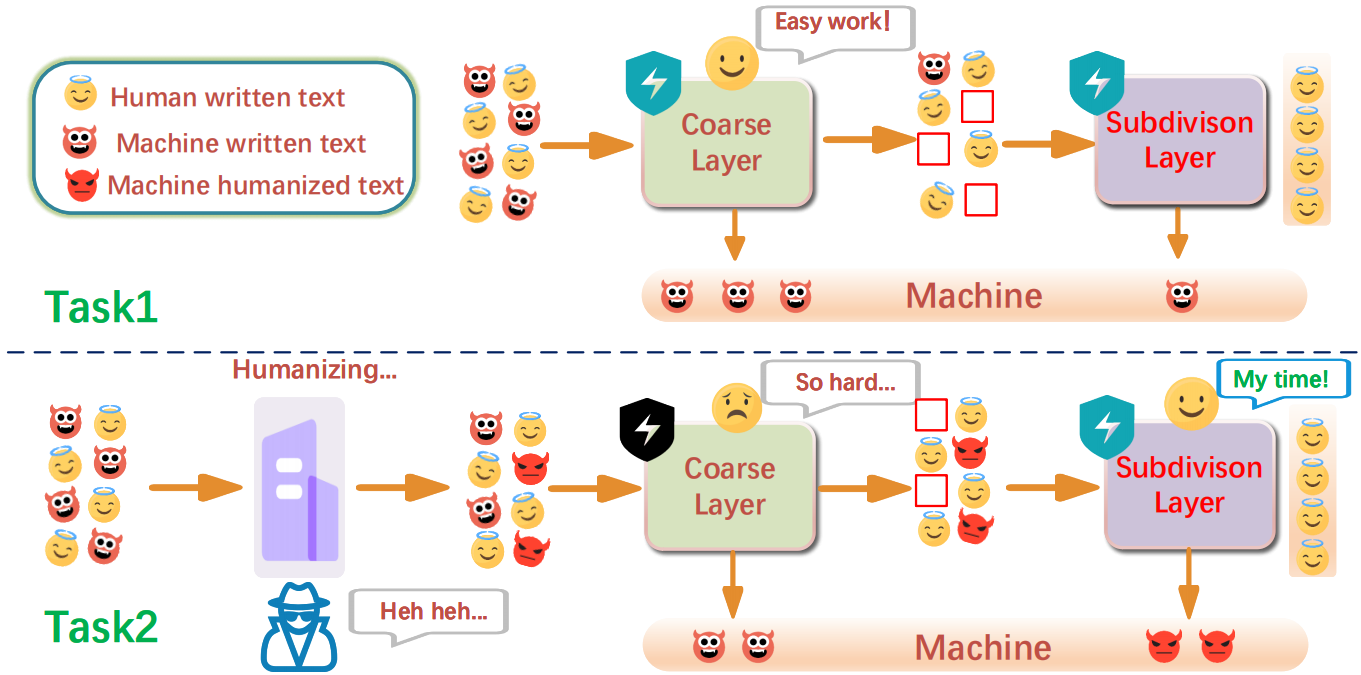
\includegraphics[width=0.9\linewidth]{pics/first-frame.png}
    \caption{HiGraDe's framework overview under two scenarios. (a) Task 1: detecting human texts and machine texts. (b) Task 2: detecting human texts and humanized machine texts, original machine texts are also included. Task 1 is simple and traditional while Task 2 is more complex and realistic.}
\label{fig:method}
\end{figure*}
	The explosive rise of LLMs~\greenCitep{Claude2024,deepseekai2025,geminiteam2024geminifamilyhighlycapable} makes it easy for people to get machine-generated texts. Just like a coin which has two sides, new problems emerge when the text generation function of LLMs facilitates people's work and life. Researchers have demonstrated various malicious applications of LLMs, including academic fraud~\greenCitep{Perkins2023}, spam generation, and false information dissemination~\greenCitep{hazell2023spear,Weidinger2022taxonomy}. In order to prevent machine-generated texts from leaning into the wrong direction, machine-generated text detectors (AI text detectors) come into being to correct the development of LLMs. Existing detectors include those based on statistics and mathematics~\greenCitep{mitchell2023detectgpt,tian2023gptzero}, watermarks~\greenCitep{gu2022watermarking,kirchenbauer2023watermark}, classifiers~\greenCitep{guo2023simpleai,wang2023seqxgpt}, to name a few. Among them, a considerable number of detectors judge whether the text is generated by machine based on the comparison of the final text's score with a certain threshold. For instance, when the test score of a text is greater than 0.5, it is considered to be written by a machine, otherwise it is considered to be written by a human. However, as large quantities of machine texts become easier to obtain and the humanizing methods become more diverse~\greenCitep{zhou2024navigatingshadows,huang2024ai}, it is not enough for detectors to depend solely on this monolithic threshold-based scoring mechanisms, and further improvement is needed.

	There are many ways of machine humanizing methods at present, such as simulating human spelling errors, word replacement, sentence back translation and so on, which can be roughly divided into four levels: character, word, sentence, and paragraph~\greenCitep{zhou2024navigatingshadows}. The vulnerability of detectors in the face of these attacks has also been pointed out by many researchers~\greenCitep{dugan2024raid,krishna2024paraphrasing}. Since single-stage detection can be easily bypassed by humanized machine texts, we believe it is necessary to conduct a dual stage and coarse-to-fine detection. To detailedly speak, when the scores of texts are within the machine category, these texts are unhumanized and easily detectable machine texts so the detection results are directly reached. When the texts' scores are within the human category, the texts may not only be human written, but also humanized machine texts, and a fine-grained detection is required. In other words, we add an extra gate to the detector, so that humanized machine texts not only need to pass the coarse detection, but also have to undergo an extra fine-grained inspection with multi-granularity contrastive learning, which greatly reduces the possibility of machine texts evading detection and improves the robustness of detector in the face of attacks.

	% We draw inspiration from the work of Concone~\greenCitep{Concone2023SpADe}, who divides spam detection into multiple stages by introducing bayesian classifier to quickly filter simple samples and costly Random Forest only for difficult samples. 
	Our detector, HiGraDe, consists of two layers. For the coarse screen layer, it is trained based on a general classifier framework, while for the subdivision layer, its training data comes from samples judged by the coarse screen layer as human writing (including human writing samples and humanized machine samples). In order to further distinguish human samples and machine samples humanized at different levels, we prescribe the right medicine by using multi-granularity contrastive learning to learn the similarities and differences between them. Concretely, for machine texts using the same humanizing method, their distance in the sample space should be close, while the distance from texts using different humanizing methods should be far; for texts humanized at the same level, their distances in the sample space should be close while far from samples humanized at other levels; for machine texts humanized at different levels along with original machine texts, their distances in the sample space should be close to each other and far from human texts. The final result can be obtained by integrating the results of the coarse detection and the fine-grained detection, which shows the vulnerability of the coarse screen layer (as a representative of the current common detectors) in the face of diversified attacks, the necessity and effectiveness of the subdivision layer, and the excellent performance of our detector that ultimately exceeds the baseline.
	
	We not only propose a new detector with good performance, but also provide a new training paradigm for subsequent AI text detectors. While for existing AI text detectors, the subdivision layer can serve as a backup in the face of large-scale humanized machine texts detection, providing them with a possible plug-and-play patch to further improve their robustness.
	
	In short, our work is multifaceted and can be summarized as follows:
	\begin{itemize}
		\item We propose a new framework for training detectors, with coarse stage targeting at detecting original machine texts and subdivison stage focusing on humanized machine texts, providing ideas for detector designers to resist the humanizing attacks.
		\item We use multi-granularity contrastive learning in subdivision layer to achieve distinction between human texts and machine texts humanized at different levels, which can also be used as a plug-and-play patch to improve the robustness of existing detectors.
		\item We conduct extensive experiments on two tasks of detecting original machine texts and humanized machine texts, results show that our detector has achieved State-Of-The-Art (SOTA) performance, we also apply our subdivision layer to current detectors and find improvement of F1-score up to 30\%.
	\end{itemize}

	\section{Related Works}
	\paragraph{Multi-stage detection.}
	The advantage of multi-stage detection is that it can subdivide the detection process and make it more granular. Jiang~\greenCite{jiang2024Staged} and Feng~\greenCite{siyue2024fire} divide the software vulnerability detection process into coarse-grained detection and fine-grained positioning. Cao~\greenCite{Cao2024RRPU} proposes a two-stage tax evasion detection. Concone~\greenCite{Concone2023SpADe} uses low-cost computing features to quickly filter easy-to-classify samples in spam detection and only performs fine-grained distinction on difficult samples. Duan~\greenCite{duan2020corner} uses two classifiers to coperform object detection. The multi-stage detection framework is also widely used in detecting video event abnormality, network attack, conversation emotion, false information, and so on~\greenCite{wang2018videoabnormal,wang2025network,li2024emotion,lin2024machine,li2021cloud}.
	
	\paragraph{Humanizing methods of machine texts.} 
	Many researchers have pointed out the vulnerability of current detectors, indicating even a small perturbation attack can cause the performance of the detector to drop sharply~\greenCitep{zhou2024navigatingshadows,dugan2024raid,krishna2024paraphrasing,liu2024pecola,huang2024ai,wang2024stumblingblocks}. Specifically, Liu~\greenCite{liu2024pecola} points out that DetectGPT relies on the threshold setting of the logit regression module (coincides with our motivation), which is sensitive to the detection results, and the perturbations of deletion, duplication, insertion, replacement imposed on the test data cause the performance of AI text detector to drop significantly; Dugan~\greenCite{dugan2024raid} designs a variety of perturbations such as local vocabulary replacement, syntactic structure adjustment, semantic preservation rewriting, finding that with only 5\% of the text content being modified, the detection accuracy drops by an average of 37.2\%; Zhou~\greenCite{zhou2024navigatingshadows} concludes humanizing methods into four levels of character, word, sentence, and paragraph on a variety of detectors (we apply this idea), pointing out that current detectors need to be trained with adversarial texts. Their works show that lacerating the mask of humanized texts is an urgent affair which current detectors need to solve.
	
	
	\section{Model and Methodology}
	\subsection{Workflow Under two Scenarios}
	\label{subsec:framework}
	Zhou and Huang's work~\greenCite{zhou2024navigatingshadows,huang2024ai} extensively explore the vulnerability of detectors to different attacks. Based on their work, we classify the existing common humanizing methods into four levels of char, word, sentence, paragraph, which consistent with Zhou's summary of present attacks~\greenCite{zhou2024navigatingshadows}, detailed in Appendix \ref{appendix:humanizing methods}. We define two tasks for AI text detectors, in which Task 1 is relatively simple, Task 2 is more realistic:
	$$
	\begin{aligned}
		\text{Task 1}: \quad &\text{Detecting human texts and machine texts}\\
		\text{Task 2}: \quad &\text{Detecting human texts, machine texts and humanized machine texts}\\
	\end{aligned}
	$$
	\label{eq:tasks_define}
	
	Given a set of unhumanized machine texts $X=\{x_1,x_2,...,x_k\}$ and human writing texts set $Y=\{y_1,y_2,...,y_k\}$, where $k$ represents the number of texts, an attacker with ulterior motives may humanize the original texts of machine at character, word, sentence, or paragraph level to try to evade detection, thus there will be sets of humanized machine texts:\\
  $$
\begin{aligned}
&X_{level} = \{x'_{1}, x'_{2}, \dots, x'_{k}\} ,\quad level \in \{char,word,sentence,paragraph\}
\end{aligned}
$$
	Given a sample space S in real world detection,we have $S = X_{char} + X_{word} + X_{sentence} + X_{paragraph} + X + Y$. For a sample $s \in S$, our goal is to ultimately determine whether it is machine generated. Sample $s$ will first pass through the coarse screen layer, the final text's score is compared with the threshold and if it is in the machine range, then the conclusion that $s$ is machine generated is directly reached, indicating that some simple machine samples are successfully identified by the first layer. If the text is judged to be human written, the text may be real human text or machine written text with humanizing methods. Sample $s$ which is judged as human by the first layer will undergo the subdivision layer with multi-granularity contrastive learning for fine-grained differentiation, ultimately determining whether $s$ is indeed a humanized machine text.
	
	\subsection{Two-layer Combined Training Paradigm}
	\textbf{Blending the strengths of both——our training idea:} With Concone's work~\greenCitep{Concone2023SpADe} in spam detection and Duan's work in object detection~\greenCitep{duan2020corner} guiding the way, we leverage cross entropy and contrastive learing. For Task 1, the classifier based on cross-entropy loss has the advantages of stable optimization process, rapid convergence, and applicability to mutually exclusive scenarios~\greenCitep{Dickson2022crossentry,ma2022crossentry,wood2022biasvariance}. Therefore, we choose it as the main body in the coarse screen layer, hoping to take advantage of its strengths and filter out the original machine texts which are simple. For the more realistic task of detecting human texts and humanized machine texts (Task 2), cross-entropy loss lacks sensitivity to intra-class differences~\greenCitep{liu2016largemarginsoftmax,Sun2020circleloss}. Therefore, we introduce multi-granularity contrastive learning as the subdivision layer, hoping it can further learn the feature representation of humanized machine texts and human texts.

	In general, the coarse screen layer quickly and roughly screens texts, solving the problem that the detector based on contrastive learning has relatively high training computational overhead when directly facing large-scale text detection and limitation in learning human texts' feature representation when facing data imbalance~\greenCitep{liu2016largemarginsoftmax,sohn2016contrasive}. The subdivision layer based on multi-granularity contrastive learning, in turn, solves the problem of coarse screen layer being insensitive to intra-class differences. Therefore, our two-layer detector HiGraDe can achieve better performance in both detecting original machine texts and detecting humanized machine texts. Better performance and lower costs are the reasons we choose "two" rather than "one", shown in Figure \ref{fig:loss_compare} and Appendix \ref{sec:cost_comparison}.

	\begin{figure*}
		\centering
		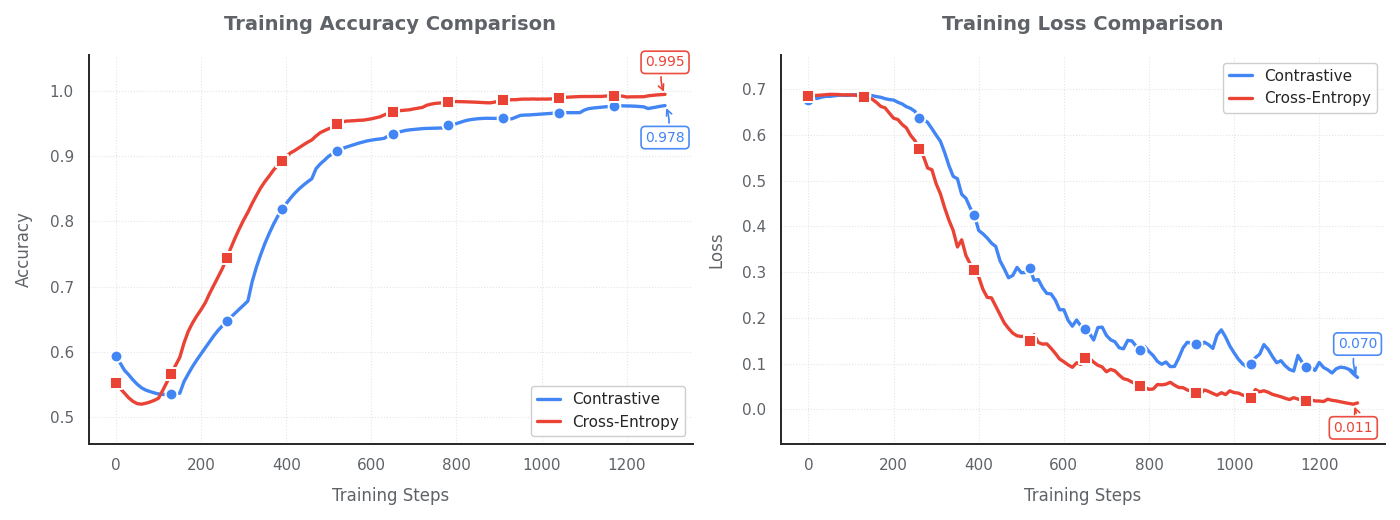
\includegraphics[width=0.9\linewidth]{pics/loss_vs.png}
		\caption{Contrastive loss VS cross-entropy loss. Model loss based on cross entropy converges faster and more stably, and its training accuracy is higher than that of the model based on contrastive learning for Task 1 and 2.}
	\label{fig:loss_compare}
	\end{figure*}
	
	\subsection{Coarse Screen Layer}
	\label{sec:first_stage}
	The coarse screen layer is a traditional classifier-based detector. Its purpose is to perform coarse-grained screening of input batch texts. This layer can also be used as a representative of the current detector that has not been specially trained with text perturbations. A good coarse screen layer should be able to filter out most of the original machine texts that have not been humanized. Its loss function is as follows,in which $l$ represents true label, $p$ represents predicted label:
  \begin{equation}
    \begin{aligned}
        \label{eq:loss_ce}
        \mathcal L_{ce}=-\frac{1}{N}\displaystyle\sum_{i=1}^N l_i\cdot log(p_i)+(1-l_i)\cdot log(1-p_i),
    \end{aligned}
\end{equation}
For input $s \in S$, the text encoding $\Phi(s)$, the output is:
\begin{equation}
	\label{ineq:seq_equal}
		Prediction(s) = 
		\begin{cases}
			human, score(\Phi(s))>threshold \\
			machine, scores(\Phi(s)) < threshold
		\end{cases}
	\end{equation}

	
	\subsection{Subdivision Layer}
	\label{sec:second_stage}
	\begin{figure*}
    \centering
    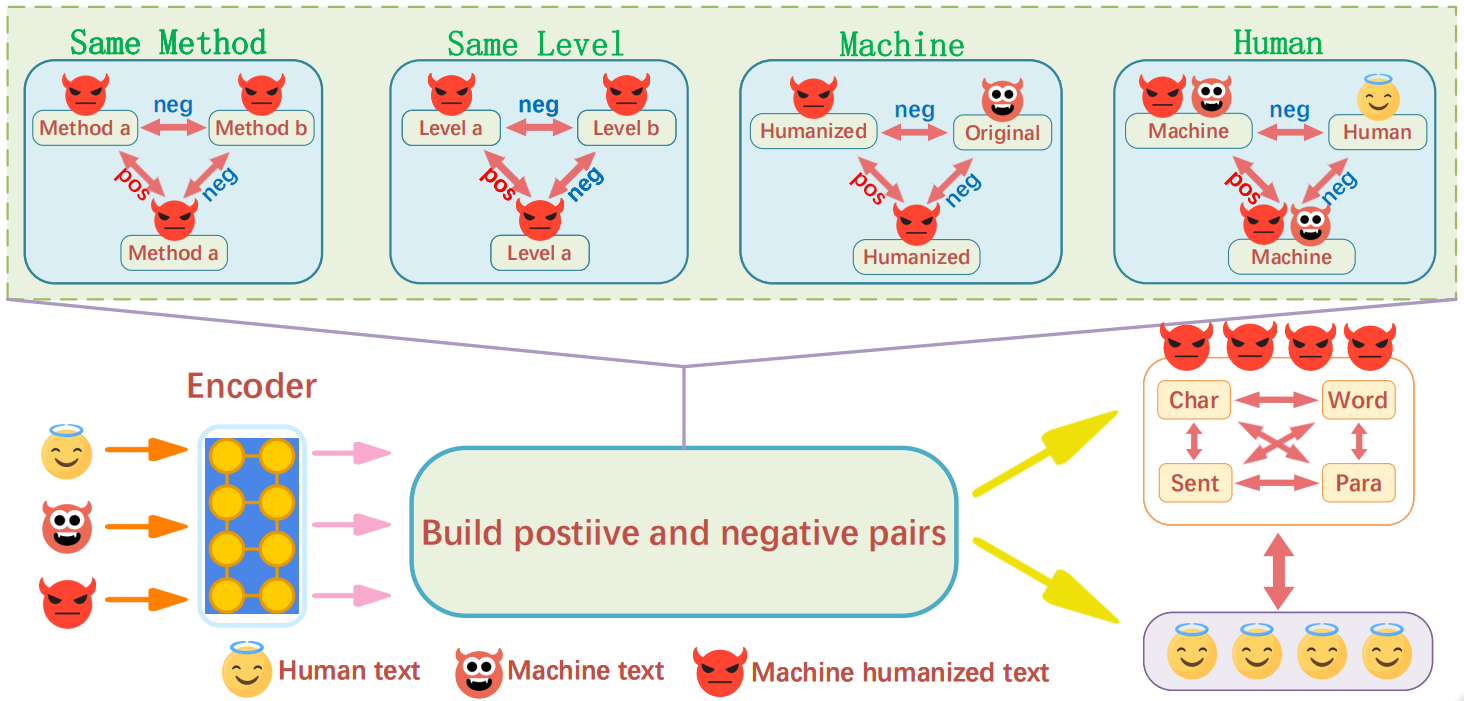
\includegraphics[width=0.9\linewidth]{pics/second-frame.png}
    \caption{Overview of the subdivision layer. After the filtered texts are encoded by the encoder, their deeper features are learned through multi-granularity contrastive learning, which pulls in the same positive samples and pushes away the negative samples to distinguish human texts and machine texts.}
\label{fig:second-detector}
\end{figure*}
	As elaborated in subsection \ref{subsec:framework} and Figure \ref{fig:method}, there are three levels of multi-granularity contrastive learning in the subdivision layer: machine texts using the same humanizing method and machine texts with different humanizing methods, machine texts using the same level of humanizing method and machine texts with different levels of humanizing methods (not humanized is seen as a special level of humanizing method), human texts and machine texts. Given a text label triple $(p, q, l)$, where $p$ represents the humanizing method used, $q$ represents the level of the humanizing method, and $l$ represents the source of the sample (human or machine), we have the cosine similarity constraints, where $s_1,s_2,s_3,s_4,s_5,s_6,s_7,s_8,s_9 \in S$:
	\begin{equation}
    \label{ineq:sim_equal}
    \left\{
    \begin{array}{@{\extracolsep{\fill}}lllll}
      Sim(\Phi(s_1),\Phi(s_2))<Sim(\Phi(s_1),\Phi(s_3)),p(s_1)=p(s_2),p(s_1)\neq p(s_3)\\
      Sim(\Phi(s_4),\Phi(s_5))<Sim(\Phi(s_4),\Phi(s_6)),q(s_4)=q(s_5),q(s_4)\neq q(s_6)\\
      Sim(\Phi(s_7),\Phi(s_8))<Sim(\Phi(s_7),\Phi(s_9)),l(s_7)=l(s_8),l(s_7)\neq l(s_9)
    \end{array}
    \right.
    \end{equation}
    For contrastive learning at a specific level, we use the contrastive loss based on Guo's framework~\greenCitep{guo2024detective}, which takes the form of a negative logarithmic aggregation function, we have the loss expression Eq.~\ref{eq:loss_function}, in which $s$ represents targeted sample, $S_{K^+}$ is a set of positive samples, $S_{K^-}$ is a set of negative samples, $\tau$ is the temperature coefficient.
    \begin{equation}
      \begin{aligned}
          \label{eq:loss_function}
           \mathcal L_p= -\log \frac{\exp \left( \sum_{k \in K^+} \frac{s(p, k)}{\tau} / S_{K^+} \right)}{\exp \left( \sum_{k \in K^+} \frac{s(p, k)}{\tau} / S_{K^+} \right) + \sum_{k \in K^-} \exp \left( \frac{s(p, k)}{\tau} \right)}.
      \end{aligned}
      \end{equation}
    We take contrastive loss in label $p$ as example,label $q$ and $l$'s loss are consistent with the above equation.

    The final contrastive learning loss should be the sum of the contrastive loss at different levels above, so we have Eq.~\ref{eq:final_contrastive_loss}, where $l_i$ represents the label $l$ that whether the $i_{th}$ sample belongs to human or machine, $K$ indicates the sum of all samples entering the subdivision layer, and $\mathcal L_l$, $\mathcal L_p$, and $\mathcal L_q$ represents the loss of the subdivision layer at above level:
    \begin{equation}
      \begin{aligned}
      \label{eq:final_contrastive_loss}
      \mathcal L_{contrastive-tot} = \displaystyle\sum_{i=1}^K l_i \cdot \mathcal L_{l-human} + (1 - l_i) \cdot (\mathcal L_p + \mathcal L_q + \mathcal L_{l-machine} ).
      \end{aligned}
  \end{equation}
  Through multi-granularity contrastive loss function propagation, the model can distinguish the differences between machine texts humanized at different levels and the similarities between machine texts humanized at the same level in a fine-grained manner. We introduce the cross-entropy loss function Eq.~\ref{eq:loss_ce} to drive the model to improve performance in the final binary classification task, the final loss is:
  \begin{equation}
    \begin{aligned}
        \label{eq:loss_overall}
        \mathcal L_{final-loss}=\mathcal L_{contrastive-tot} + \mathcal L_{ce}.
    \end{aligned}
    \end{equation}

	\section{Experiments}
	\subsection{Experimental Setup}
	\label{sec:experimental_setup}
	\paragraph{Datasets.} 
	 We use three datasets that are widely used for detector training and detection. Detailed dataset information in Appendix \ref{subsec:dataset_appendix}. \textbf{HC3}~\greenCitep{guo2023simpleai}: A high-quality dataset specifically for fine-tuning dialogue models, containing QA question-answer pairs in multiple fields, each question corresponds to at least one human answer and one machine-generated answer, focusing on multiple open-ended questions such as finance and medicine. \textbf{SeqXGPT-Bench}~\greenCitep{wang2023seqxgpt}: A benchmark dataset designed specifically for sentence-level AI generated text detection tasks, containing text generated from multiple LLMs (such as GPT-2, GPT-Neo, GPT-J, LLaMa, and GPT-3). The dataset uses feature alignment design to align word-level log probabilities to a common vocabulary. \textbf{CheckGPT}~\greenCitep{liu2024checkgpt}: This dataset contains 900,000 samples, generated by ChatGPT based on prompts, covering multiple fields such as news, reviews, and literatures.

	\paragraph{Evaluating Metrics.}
	In order to systematically and thoroughly evaluate our work and the work of others, we use Accuracy (ACC), F1-score (F1), and Recall as the standard. ACC: The proportion of correctly predicted samples to the total number of samples, which directly reflects the overall prediction accuracy of the model, but may be distorted when the categories are unbalanced; Recall: The proportion of correctly predicted samples among samples that are actually positive, which measures the model's coverage of positive samples, but may have a high false alarm rate; F1: The harmonic average of precision and recall, which balances Precision and Recall and avoids the one-sidedness of a single indicator. We use the three in combination with the hope of evaluating model performance more comprehensively.
	
	\paragraph{Baseline Detectors.}
	To verify the effectiveness of our method, we select the following five representative detectors as baselines and compare them with HiGraDe. Considering that machine texts may be humanized in reality, we specially select three baseline detectors that have gone through adversarial training or text perturbation training. \textbf{SimpleAI}~\greenCitep{guo2023simpleai}: Fine-tune the pre-trained RoBERTa model, filter the patterned words in the training data to improve generalization ability, and add sentence-level data to enable the model to capture local features. \textbf{Watermark}~\greenCitep{kirchenbauer2023watermark}: The watermark embeds the signal by biasing the "green token list" at generation time, and the detector counts the actual number of green tokens in the texts. It is completely independent of the generation model, avoiding the overhead of traditional model training while ensuring the robustness and interpretability of the detection. \textbf{CoCo}~\greenCitep{liu2023coco}: By constructing a coherence graph to capture the entity interaction structure of the text and introducing a supervised contrastive learning framework, the model's understanding of language patterns is enhanced. \textbf{RADAR}~\greenCitep{hu2023radarrobustaitextdetection}: Using the adversarial learning framework of generator and discriminater along with some instruction tuning, model shows excellent robustness and transferability. \textbf{PECOLA}~\greenCitep{liu2024pecola}: The noise introduced by random perturbations is reduced through selective perturbation strategies, the key features of the text are retained, and the contrastive learning strategy is further used to enhance the robustness.

	\subsection{Results and Analysis}
	In order to better illustrate the effectiveness of our method, we retrain the existing baseline detectors on the three datasets of HC3, SeqXGPT and CheckGPT according to the method described in their papers and compare them with HiGraDe. Among them, RADAR does not provide source code, so we use the API they provide. In addition, the watermark-based detector does not need to be trained, its processing work is to add watermarks to the input dataset. We first conduct tests on Task 1. The results are shown in Table \ref{tab:combined_results}. For HC3 and SeqXGPT datasets, our method outperforms all baseline detectors in all evaluating metrics. For the CheckGPT dataset, we achieve the best in F1, ACC, and also achieve the second best in overall recall. Further, using the comprehensive evaluating metric of F1 to illustrate, HiGraDe is 0.72\% higher than the second place on the SeqXGPT dataset and 4.11\% higher than the second place on the CheckGPT dataset. For the HC3 dataset, although it is released relatively early and the recognition difficulty may be relatively low, all baseline detectors perform well, HiGraDe still achieves a certain breakthrough with F1 0.54\% higher than the second place. The above results show that the cross-data adaptability of our two-layer framework is commendable, and acquires the most advanced performance in Task 1.
	\begin{figure*}
		\centering
		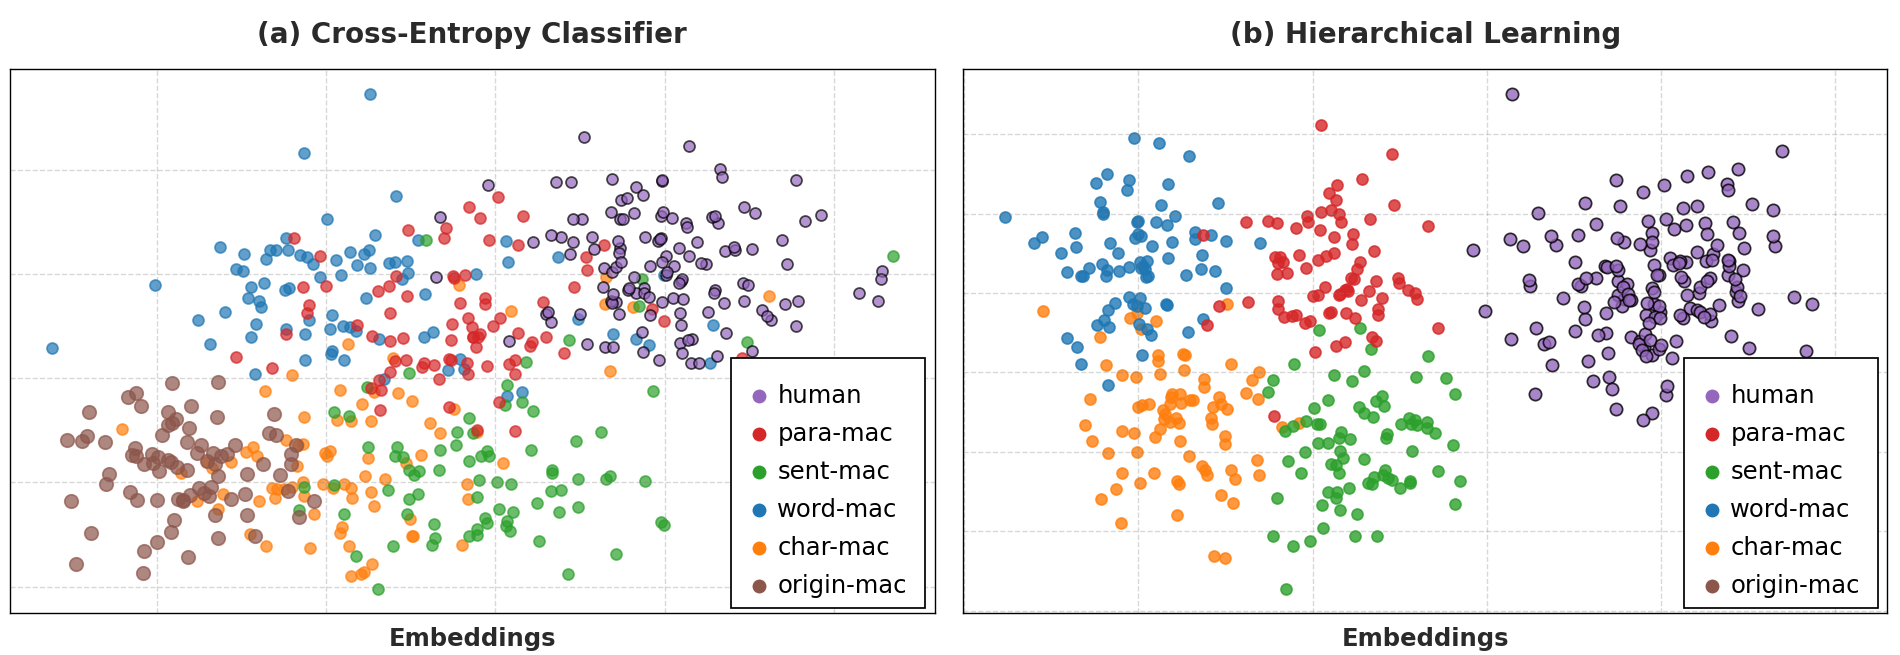
\includegraphics[width=\linewidth]{pics/classify.png}
		\caption{Illustration of contrastive learning and cross entropy on final texts' embeddings. Para-mac reffers to text using humanizing method of paragraph level, rest are the same.}
	\label{fig:classify_compare}
	\end{figure*}
	\begin{table*}[ht]
    \centering
    \resizebox{0.9\textwidth}{!}{ 
    \renewcommand{\arraystretch}{1.1}
    \begin{tabular}{llccc|ccc}
        \toprule
        \multirow{2}{*}{Dataset} & \multirow{2}{*}{Detectors} & \multicolumn{3}{c}{Origin} & \multicolumn{3}{c}{Humanized} \\
        \cmidrule(lr){3-5} \cmidrule(lr){6-8}
        & & Recall & F1 & ACC & Recall & F1 & ACC \\
        \midrule
        
        \multirow{6}{*}{HC3}
        & SimpleAI & 94.32 & 94.31 & 94.32 & 71.58 & 79.25 & \underline{96.44} \\
        & Watermark & 94.75 & 95.13 & 94.88 & 76.03 & 69.05 & 55.16 \\
        & CoCo & \underline{99.31} & 98.30 & 98.42 & 58.18 & \underline{95.09} & 94.44 \\
        & RADAR & 89.57 & 90.39 & 89.57 & \underline{79.20} & 89.40 & 81.75 \\
        & PECOLA & 99.25 & \underline{99.24} & \underline{99.23} & 64.03 & 70.59 & 95.44 \\
        & HiGraDe & \textbf{99.78} & \textbf{99.78} & \textbf{99.80} & \textbf{96.26} & \textbf{95.99} & \textbf{99.52} \\
        \cline{1-8}
        
        \multirow{6}{*}{SeqXGPT}
        & SimpleAI & 94.38 & 94.36 & 94.37 & 81.74 & 86.18 & 97.04 \\
        & Watermark & \underline{96.30} & \underline{95.92} & \underline{96.07} & 76.22 & 68.80 & 54.61 \\
        & CoCo & 82.36 & 79.54 & 80.67 & \underline{93.65} & \underline{93.06} & \underline{98.16} \\
        & RADAR & 61.15 & 54.16 & 61.37 & 66.77 & 72.08 & 58.51 \\
        & PECOLA & 90.83 & 90.82 & 90.82 & 74.98 & 80.30 & 96.06 \\
        & HiGraDe & \textbf{96.70} & \textbf{96.64} & \textbf{96.66} & \textbf{97.23} & \textbf{94.02} & \textbf{99.21} \\
        \cline{1-8}
        
        \multirow{6}{*}{CheckGPT}
        & SimpleAI & 87.82 & \underline{88.78} & \underline{88.77} & \underline{88.58} & 70.21 & 90.52 \\
        & Watermark & \textbf{97.06} & 72.26 & 75.69 & 76.54 & 69.56 & 56.22 \\
        & CoCo & 84.90 & 85.97 & 84.55 & 85.63 & \textbf{98.21} & 96.60 \\
        & RADAR & 63.26 & 63.01 & 63.04 & 72.71 & 75.35 & 61.94 \\
        & PECOLA & 87.16 & 86.79 & 86.82 & 69.14 & 75.63 & \underline{96.90} \\
        & HiGraDe & \underline{93.33} & \textbf{92.89} & \textbf{93.55} & \textbf{96.08} & \underline{95.71} & \textbf{99.63} \\
        \bottomrule
    \end{tabular}
			}
			\caption{Combined performance results across original and humanized datasets. The best number is highlighted in \textbf{bold}, while the second best one is \underline{underlined}.}
			\label{tab:combined_results}
	\end{table*}

			To further illustrate that our two-layer training paradigm can train a more robust detector, we humanize the machine texts in the HC3, SeqXGPT and CheckGPT datasets at different levels, and retrain the baseline detector based on the humanized dataset to compare with HiGraDe. Results correspond to the humanized column in Table \ref{tab:combined_results}. Our detector HiGraDe has achieved SOTA performance on the three humanized datasets. In terms of recall, F1, and ACC, HiGraDe is 17.06\%, 0.90\%, and 3.08\% higher than the second place on the HC3 dataset, and 3.58\%, 0.96\%, and 1.05\% higher than the second place on the SeqXGPT dataset. On the CheckGPT dataset, recall and ACC are both the first place, and F1 reaches the runner-up performance. Furthermore, for the detector CoCo, which also has outstanding performance, although its performance on the CheckGPT dataset is comparable to ours, it relies on the extraction of entities in texts and the construction of a coherence graph. If the machine texts are relatively concise and short, its performance will suddenly drop because of the failure in building coherence graphs. In our experiments on the HC3 dataset, we find that 10,083 out of 24,000 data do not have corresponding coherence graphs, which leads to a sudden collapse of CoCo's recall metric (58.18\%). Overall, HiGraDe performes well on all three datasets, and demonstrates excellent generalization and robustness in Task 2.

			\begin{figure*}
				\centering
				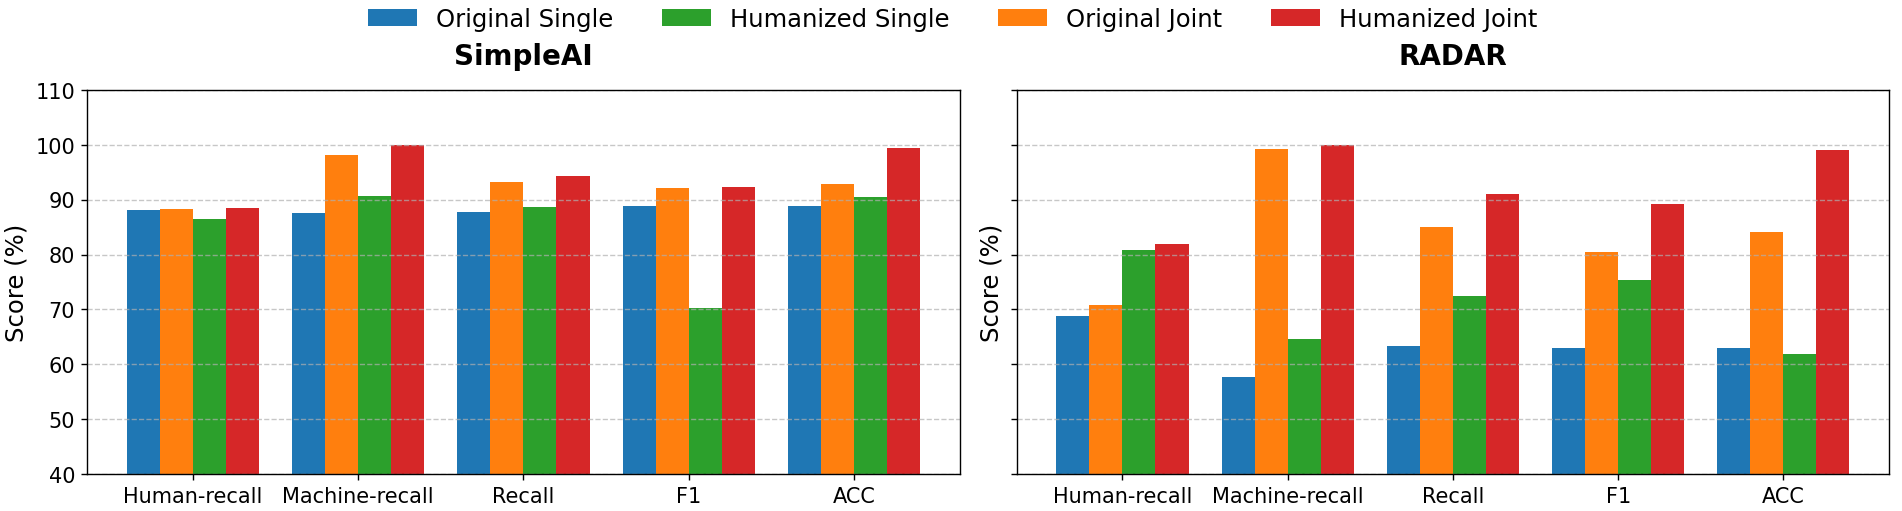
\includegraphics[width=0.9\linewidth]{pics/two-patch.png}
				\caption{Illustration of "patch" result for baseline detectors SimpleAI and RADAR on CheckGPT dataset, original (humanized) represents the original (humanized) dataset, single represents the original detector, joint represents detecor using our patch. Results prove that our patch can effectively improve the performance of the current baseline detectors. Detailed results are shown in Appendix \ref{sec:detailed_patch_results}.}
		\label{pic:patch_result}
		\end{figure*}

					\begin{table*}[ht]
						\centering
						\resizebox{0.9\textwidth}{!}{ 
						\renewcommand{\arraystretch}{1.1}
						\begin{tabular}{lllccccc}
						\toprule
						\multirow{2}{*}{Method} & \multirow{2}{*}{Type} & \multirow{2}{*}{Detectors} & \multicolumn{5}{c}{Metrics} \\
						\cmidrule(lr){4-8}
						& & & Human-recall & Machine-recall & Recall & F1 & ACC \\
						\midrule
						
						\multirow{4}{*}{Contrastive Learning} 
						& \multirow{2}{*}{Original} 
						& Single & \textbf{89.48} & 92.25 & 90.86 & 90.45 & 91.44 \\
						& & Joint & 88.13 & \textbf{98.99} & \textbf{93.56} & \textbf{93.15} & \textbf{93.77} \\
						\cline{2-8}
						
						& \multirow{2}{*}{Humanized}
						& Single & \textbf{86.90} & 94.13 & 90.52 & 55.78 & 93.81 \\
						& & Joint & 85.91 & \textbf{99.80} & \textbf{92.86} & \textbf{90.39} & \textbf{99.18} \\
						\midrule
						\midrule
						\multirow{4}{*}{Fine-tuned DeBERTa}
						& \multirow{2}{*}{Original} 
						& Single & 94.17 & 89.17 & 91.67 & 91.62 & 91.70 \\
						& & Joint & \textbf{94.43} & \textbf{90.09} & \textbf{92.26} & \textbf{91.92} & \textbf{92.05} \\
						\cline{2-8}
						& \multirow{2}{*}{Humanized}
						& Single & 91.64 & 91.57 & 91.60 & 50.12 & 91.65 \\
						& & Joint & \textbf{93.36} & \textbf{99.97} & \textbf{96.67} & \textbf{95.32} & \textbf{99.60} \\
						
						\bottomrule
						\end{tabular}
						}
						\caption{Performance results of "patching" results for contrastive learning and fine-tuned DeBERTa.}
						\label{tab:combined_patch_results}
				\end{table*}
				We further explore the effect of our framework in "patching" existing detectors, given that the coarse screen layer plays an important role in the overall detection effect, its initial screening of data directly affects the training and detection of the subdivision layer. We replace the first layer based on traditional classification loss with fine-tuned DeBERTa (Wang's framework)~\greenCitep{wang2024stumblingblocks} and detecor based on supervised contrastive learning (Chen's framework)~\greenCitep{Chen2022contastive}, along with baseline detectors SimpleAI~\greenCitep{guo2023simpleai} and RADAR~\greenCitep{hu2023radarrobustaitextdetection}.
				
				Results are shown in Table \ref{tab:combined_patch_results} and Figure \ref{pic:patch_result}. For the existing detectors based on contrastive learning, the F1 reaches 90.45\% and the ACC reaches 91.44\% in Task 1, which shows that a relatively ideal effect has been achieved in the first layer. On this basis, we further use our subdivision layer to play the role of the second gate in the hope of achieving a more refined effect. The results are consistent with our expectations. The patched detector further improves the F1 to 93.15\% and the ACC to 93.77\%. For Task 2, the detector without the patch has only 55.78\% of F1, which shows a large number of humanized machine texts are misjudged as human. However, using our patch, a second checkpoint is set up in time to capture these humanized texts that bypass detection, and the F1 score is increased by a huge span of 34.61\% to 90.39\%. This further proves our original intention of using two-layer detection: To give the existing detector robustness when facing large-scale humanized machine texts, and further improve its recognition ability of machine texts so that it can effectively capture both original and humanized texts. Overall, by applying our patch, we achieve a significant improvement in most evaluation metrics, with only a minor sacrifice of 1\% in human texts recall, resulting in a substantial overall performance optimization.
	
	\subsection{Ablation Studies}
		 First, we directly apply the first layer, the second layer, and two-layer detecor HiGraDe to Task 1 (Original) and Task 2 (Humanized). Results are shown in Table \ref{tab:combined_ablation_results}. For Task 1, coarse screen layer performes well overall, which confirms its applicability and practicality in the simple binary classification task of detecting human texts and original machine texts. The subdivision layer performes relatively averagely, with an F1 of 63.88\% and an ACC of only 47.18\%. This phenomenon is well explained: second layer is trained with samples screened by the first layer as data set. If it is directly applied to the original texts detection, the effect may not be satisfactory. This is also the reason why the F1 and ACC scores of the second-stage detector plummets in Task 2. For task 2, although the coarse screen layer bears a good recall rate, combined with the imbalance of the dataset under this task (the humanizing methods of machine texts are varied, Appendix \ref{subsec:dataset_appendix}) and its poor performance in F1 score (55.78\%), indicating that it will misjudge a large number of humanized machine texts as human, which is consistent with our expectation that "the robustness of the first layer is fragile when facing large-scale humanized texts", and is one of the reasons why we introduce the subdivision layer.

	\begin{table*}[ht]
    \centering
    \resizebox{0.8\textwidth}{!}{ 
    \renewcommand{\arraystretch}{1.1}
    \begin{tabular}{llccc|ccc}
    \toprule
    \multirow{2}{*}{Type} & \multirow{2}{*}{Detectors} & \multicolumn{3}{c}{Direct Apply} & \multicolumn{3}{c}{Direct Train} \\
    \cmidrule(lr){3-5}\cmidrule(lr){6-8}
    & & Recall & F1 & ACC & Recall & F1 & ACC \\
    \midrule
    
    \multirow{3}{*}{Original} 
    & First      & 90.52 & 90.07 & 90.60 & 88.75 & 90.07 & 90.60 \\
    & Second     & 87.15 & 63.88 & 47.18 & 88.16 & 87.09 & 88.40 \\
    & Combined   & \textbf{93.33} & \textbf{92.89} & \textbf{93.55} & \textbf{93.33} & \textbf{92.89} & \textbf{93.55} \\ 
    \cline{1-8}
    
    \multirow{3}{*}{Humanized}
    & First      & 91.46 & 57.22 & 94.05 & 83.43 & 74.95 & 96.94 \\
    & Second     & 89.67 & 8.50  & 5.15  & 88.42 & 85.51 & 97.83 \\
    & Combined   & \textbf{96.08} & \textbf{95.71} & \textbf{99.63} & \textbf{96.08} & \textbf{95.71} & \textbf{99.63} \\
    \bottomrule
    \end{tabular}
    }
    \caption{Merged results of ablation study. Direct Apply represents results from direct application, Direct Train represents results from direct training.}
    \label{tab:combined_ablation_results}
\end{table*}
		
			To further verify the effectiveness of the two-layer joint training framework, we directly trains the first layer and second layer on the CheckGPT dataset in Task 1 and 2. For the coarse screen layer, even after training with humanized texts, it still has the phenomenon of "wrongly accusing good guys" when detecting humanized machine texts, which reveals the limitations of single stage detection in adversarial scenarios. For subdivision layer, in Task 1, its multi-granularity contrastive learning will degenerate into single-granularity contrastive learning, while in Task 2, its ability to discriminate human texts is slightly weak due to the fact that in the face of a variety of large-scale humanized machine texts in reality, contrastive learning learns limited features of human texts.

			Overall, whether it is detecting original machine text or humanized machine text, whether it is directly applied or trained, deleting any component will lead to a decrease in the overall performance of HiGraDe and it is undoubtedly worthwhile to sacrifice the recall rate of human texts slightly in exchange for a significant improvement in overall performance.
			
	\section{Conclusion}
	In this paper, we propose a coarse-to-fine AI generated text detector model and a novel training paradigm. The coarse screen layer quickly screens the original machine texts, and the subdivision layer uses multi-granularity contrastive learning to carefully distinguish different levels of humanized machine texts. Our detector HiGraDe has achieved SOTA performance in the task of detecting human texts from original machine texts and the more realistic task of detecting human texts from humanized machine texts, proving the effectiveness of each component and the correctness of the "blending the strengths of both" training paradigm. Moreover, our subdivision layer is a plug-and-play patch that can be easily applied to existing detectors to further improve their performance. We hope HiGraDe can better assist AI text detection in real life, and that this hierarchical and multi-granularity contrastive learning framework can bring new maps and ideas to researchers in this field.

	\newpage
	\bibliography{custom}
	
	\newpage
	\appendix
	\section{Broader Impacts}
	\label{sec:Impacts}
	The rapid development of LLMs has enabled a large amount of machine-generated texts to be obtained quickly and at low cost. Given that it may lead to academic fraud, phishing emails, the spread of false information and other problems, detecting and monitoring AI-generated texts is undoubtedly a top priority. However, due to the fragility of current AI content detectors and the diversity of text humanizing methods, machine texts can easily bypass detection after humanizing. Therefore, the development of robust AI content detectors is urgent. Our paper introduces a new robust AI content detector training paradigm, which demonstrates SOTA performance in multiple benchmarks. These advances will bring the green development and use of LLMs with new power. In addition, our second-stage detector can be used as a "patch" to further improve the performance of current detectors when facing large-scale humanized machine texts, which shows that our method has broad prospects for practical application and rich significance.

	
	\section{Limitations and Future Work}
	In this paper, we take into consideration that machine texts may use different humanizing methods to evade the detector and thus use multi-granularity contrastive learning to strengthen the detector in a targeted manner. However, the original machine texts generated by different models often has certain differences, which may affect the performance of the detector. In addition, we did not introduce some latest humanizing strategies (such as adding emoticons to machine texts) and did not train on a larger corpus. In the future, we will continue to work in this direction and further improve the performance of the model.

	\section{Detailed Humanizing Methods and Its Levels}
	\label{appendix:humanizing methods}
	Following Zhou's work~\cite{zhou2024navigatingshadows}, four types of humanizing methods are classified below:
	\begin{enumerate}
		\item \textbf{char level}: Attacks at this level include space deletion, space addition~\greenCitep{cai2023evadechatgpt}, capitalization typo simulation, punctuation deletion, and random word merging.
		\item \textbf{word level}: Attacks at this level include keyboard spelling errors, which replace characters in similar keyboard positions; swaping adjacent characters, inserting irrelevant characters, and deleting specific characters, thereby simulating human negligence when typing; word spelling errors, which simulate users' incorrect spelling of words through a predefined spelling error dictionary; adverb perturbations, which randomly insert relevant adverbs before verbs in the original text; word replacement, which uses the BERT model~\greenCitep{devlin2019bert} to replace words in the text with synonyms.
		\item \textbf{sentence level}: Attacks at this level include adding irrelevant sentences; repeating parts of sentences; randomly selecting sentences for back-translation; and sentence-level replacement, which randomly masks 2 to 5 sentences in the original text and replaces them using the BART-large model~\greenCitep{lewis2020bart}.
		\item \textbf{paragraph level}: Attacks at this level include rewriting using the Dipper interpreter~\greenCitep{krishna2024paraphrasing}; back-translation using the Helsinki-NLP model~\greenCitep{tiedemann2020opus}; and rearrangement of paragraph structure.
	\end{enumerate}
	Given original machine texts $X$, we thus have humanized machine texts set:
	$$
	\begin{aligned}
		&X_{humanized}=\{X_{char},X_{word},X_{sent},X_{para}\}
	\end{aligned}
	$$
	which is illustrated in section \ref{subsec:framework}.

	\section{Detailed Construction of Dataset}
	\label{subsec:dataset_appendix}
	\begin{table*}[ht]
    \centering
    \begin{minipage}[t]{0.58\textwidth} 
        \centering
        \resizebox{\textwidth}{!}{ 
            \renewcommand{\arraystretch}{1.1}
            \begin{tabular}{lccc}
                \toprule
                \multirow{2}{*}{\large Dataset} & \multirow{2}{*}{\large Train} & \multirow{2}{*}{\large Test} & \multirow{2}{*}{\large Valid} \\
                 & & & \\
                \midrule
                CheckGPT & (2000,2000) & (1921,2078) & (2500,2500) \\
                HC3      & (5000,5000) & (5000,5000) & (2000,2000) \\
                SeqXGPT  & (2467,2533) & (1928,1872) & (1005,995)  \\
                \bottomrule
            \end{tabular}
        }
        \caption{Detailed composition of the dataset for detecting human texts and original machine texts.}
        \label{tab:detailed_original_datasets}
    \end{minipage}
    \hfill 
    \begin{minipage}[t]{0.38\textwidth}
        \centering
        \resizebox{\textwidth}{!}{
            \renewcommand{\arraystretch}{1.1}
            \begin{tabular}{lcc}
                \toprule
                \multirow{2}{*}{Watermark} & \multirow{2}{*}{Human} & \multirow{2}{*}{Machine} \\
                 & & \\
                \midrule
                CheckGPT & 566 & 570 \\
                HC3      & 438 & 538 \\
                SeqXGPT  & 600 & 520 \\
                \bottomrule
            \end{tabular}
        }
        \caption{Detailed composition of the dataset for watermarks.}
        \label{tab:watermark_original_datasets}
    \end{minipage}
\end{table*}

\begin{table*}[ht]
	\centering
	\begin{minipage}[t]{0.58\textwidth} 
			\centering
			\resizebox{\textwidth}{!}{ 
					\renewcommand{\arraystretch}{1.1}
					\begin{tabular}{lccc}
							\toprule
							\multirow{2}{*}{\large Dataset} & \multirow{2}{*}{\large Train} & \multirow{2}{*}{\large Test} & \multirow{2}{*}{\large Valid} \\
							 & & & \\
							\midrule
							CheckGPT & (500,8500) & (1101,23887) & (500,8490) \\
							HC3      & (500,7500) & (1500,22500) & (500,7500) \\
							SeqXGPT  & (500,7500) & (1500,21004) & (500,6494)  \\
							\bottomrule
					\end{tabular}
			}
			\caption{Detailed composition of the dataset for detecting human texts and humanized machine texts.}
			\label{tab:detailed_attack_datasets}
	\end{minipage}
	\hfill 
	\begin{minipage}[t]{0.38\textwidth}
			\centering
			\resizebox{\textwidth}{!}{
					\renewcommand{\arraystretch}{1.1}
					\begin{tabular}{lcc}
							\toprule
							\multirow{2}{*}{Watermark} & \multirow{2}{*}{Human} & \multirow{2}{*}{Machine} \\
							 & & \\
							\midrule
							CheckGPT & 566 & 8550 \\
							HC3      & 438 & 8098 \\
							SeqXGPT  & 600 & 520 \\
							\bottomrule
					\end{tabular}
			}
			\caption{Detailed composition of the humanized dataset for watermarks.}
			\label{tab:watermark_attack_datasets}
	\end{minipage}
\end{table*}
For the simple binary classification task of detecting human texts and original machine texts, the distribution of our samples is shown in Table \ref{tab:detailed_original_datasets}. We ensure the distribution of human texts and machine texts is approximately 1:1. The two-tuple (human, machine) in the table represents the number of human texts and the number of machine texts. For the watermark detector, since it focuses on the hidden singal embedded in the data and does not require training, it only needs to build a test set. While it takes a long time to process the watermark on the dataset, we did not generate a large test set. The data are shown in Table \ref{tab:watermark_original_datasets}.
For the more realistic task of detecting human texts and humanized machine texts, the distribution of our samples is shown in Table \ref{tab:detailed_attack_datasets}. We select 500 human texts and 500 original machine texts from the dataset respectively, and perform 16 humanizing methods on the machine texts at the character, word, sentence, and paragraph levels, thereby constructing a perturbation dataset containing human texts, original machine texts, and humanized machine texts. Therefore, the perturbed datasets are mostly composed of machine texts, which are consistent with the current trend of a variety of machine text humanizing methods and a flood of generation sources. For the watermark detector, similarly, after the machine texts are injected with the watermark, we humanize them in sixteen different ways and explore whether these humanizing attacks will cause the watermark to be covered and invalid. The data distribution is shown in Table \ref{tab:watermark_attack_datasets}.

\section{Comparison of Detectors in Costs}
\label{sec:cost_comparison}
\begin{table*}[ht]
	\centering
	\renewcommand{\arraystretch}{1.1}
	\begin{tabular}{lcccc}
			\toprule
			\multirow{2}{*}{Detectors} & 
			\multirow{2}{*}{Preprocess Time} & 
			\multirow{2}{*}{Preprocess Memory} & 
			\multirow{2}{*}{Train Time} & 
			\multirow{2}{*}{Train Memory} \\
			& & & & \\
			\midrule
			PECOLA & 22:17:04 & 642 & 00:08:55 & 9228 \\
			CoCo      & 04:42:56 & 10520 & 00:33:27 & 14556 \\
			Watermark  & 153:21:22 & 1290 & 00:01:31  & 840 \\
			Contra & no need & no need & 00:12:40 & 10840 \\
			Coarse & no need & no need & 00:08:40 & 10840 \\
			Subdivision & no need & no need & 00:01:36 & 10840 \\
			\bottomrule
	\end{tabular}
	\caption{Detailed comparison of the detectors in terms of costs. Preprocess time means data should be preprocessed before training.}
	\label{tab:detailed_compare_cost}
\end{table*}
The baseline detectors SimpleAI and RADAR are similar to coarse layer (which are also the subjects of our patching experiments) thus are not considered here. Shown in Table \ref{tab:detailed_compare_cost}, Contra means we directly use contrastive learning to train the detector. The data processing and training time are formed in hour: minute :second, and the memory occupied is in MB. Watermark does not require additional training of the detector, and its training time is temporarily expressed as the detection time. We uniformly set the training batch size to 16, the training round to 15, and trained on NVIDIA RTX A6000. The high cost of contrastive learning is that it needs to calculate the similarity between all sample pairs, which has a time complexity of $O(n^2)$ while cross entropy of $O(n)$, which will mainly affect training time rather than memory usage. Compared with using contrastive learning directly, the subdivision layer only needs to process the filtered samples, and the training time is reduced from 12 minutes to 1 minute 36 seconds. In addition, although PECOLA, CoCo and Watermark have achieved good performance in detecting machine texts, their cumbersome and lengthy data preprocessing process deserves high attention and needs to be considered seriously. Taking CoCo as an example, it is slow in extracting entity graphs from texts,  takeing nearly 5 hours to extract 8,000 training samples. When large-scale machine text needs to be detected in real life, such as the 23005 samples in our test data set, its data preprocessing takes an astonishing 17 hours, shown in Table \ref{tab:detailed_COCO_cost}. These situations remind us that if we want to make an AI content detector with advanced performance and practical significance, the time issue of data processing needs to be paid great attention to.
\begin{table*}[ht]
	\centering
	\begin{minipage}[t]{0.51\textwidth} 
			\centering
			\resizebox{\textwidth}{!}{ 
					\renewcommand{\arraystretch}{1.1}
					\begin{tabular}{cccc}
							\toprule
							\multirow{2}{*}{\large PECOLA} &\multirow{2}{*}{\large Augment} & \multirow{2}{*}{\large Select} & \multirow{2}{*}{\large Total} \\
							 & & & \\
							\midrule
							Train & 00:03:44 & 22:13:20 & 22:17:04 \\
							Eval      & 00:03:16 & 19:26:45 & 19:30:01 \\
							Test  & 00:09:48 & 56:56:28 & 57:06:16  \\
							\bottomrule
					\end{tabular}
			}
			\caption{Detailed time cost for PECOLA in building train, eval and test sets. Augment means data augmentation, Select means its selecting strategy.}
			\label{tab:detailed_PECOLA_cost}
	\end{minipage}
	\hfill 
	\begin{minipage}[t]{0.45\textwidth}
			\centering
			\resizebox{\textwidth}{!}{
					\renewcommand{\arraystretch}{1.1}
					\begin{tabular}{cccc}
							\toprule
							\multirow{2}{*}{CoCo} & \multirow{2}{*}{Extract} & \multirow{2}{*}{Build} & \multirow{2}{*}{\large Total} \\
							 & & &\\
							\midrule
							Train & 04:41:04 & 00:00:31 & 04:42:56 \\
							Eval  & 02:03:20 & 00:00:23 & 02:03:43 \\
							Test  & 17:06:38 & 00:01:21 & 17:07:59 \\
							\bottomrule
					\end{tabular}
			}
			\caption{Detailed time cost for CoCo in building train, eval and test sets. Extract means extracting entity, Build means building graphs according to the extracted entities.}
			\label{tab:detailed_COCO_cost}
	\end{minipage}
\end{table*}

	\section{Machine-Generated Text Detectors}
	In order to prevent machine-generated texts from being abused, numbers of detectors have been proposed by researchers, thus consolidating the defense line of text detection. We classify the existing detectors into the following four categories:

	\textbf{Statistical and mathematical based detectors}: Using information entropy, cross perplexity, word frequency statistics and other features to perform zero-shot detection. Mithcell~\greenCite{mitchell2023detectgpt} quantifies the difference between machines and human in word selection via conditional probability curvature. Su~\greenCite{su2023detectllm} applies log-rank information to detect. Open source detecting platform GPTZero and GLTR~\greenCite{tian2023gptzero,gehrmann2019gltrstatisticaldetectionvisualization} are also included. 
	
	\textbf{Watermark based detectors}: Watermark detection algorithms in machine texts detection track the source of generated texts by embedding invisible identifiers. Representative works include:~\greenCite{gu2022watermarking,liu2024unforgeablepubliclyverifiablewatermark,hou2024clusteringbasedsemanticwatermark,lu2024entropybasedwatermarking}. Among them, Kirchenbauer~\greenCite{kirchenbauer2023watermark} adds a fixed weight to the logit value of the predefined "green word list" and determine whether the text is generated by the model by counting the proportion of green words in the texts. 
	
	\textbf{Classifier based detectors}: Researchers~\greenCite{Chen_2023,miao2024efficientdetection,mireshghallah2024smallerlanguagemodelsbetter,wang2023seqxgpt,liu2024checkgpt} typically employ RoBERTa~\greenCitep{liu2019roberta} as the backbone architecture for training supervised binary classifiers. Notable developments are seen in OpenAI's official detection toolkit~\greenCitep{solaiman2019releasestrategiessocialimpacts} and RADAR~\greenCitep{hu2023radarrobustaitextdetection}, which enhances adversarial robustness against perturbation attacks through paraphrase-based adversarial training. 
	
	\textbf{Other methods based detecors}: Soto~\greenCite{soto2024fewshotdetectionmachinegeneratedtext} uses style representations, Huang~\greenCite{huang2024ai} takes advantage of siamese neural network, Krishna~\greenCite{krishna2024paraphrasing} achieves success through retrieval methods. Zhu~\greenCite{zhu2023beatllm} innovatively queries LLM to detect LLM-generated texts.

	\section{Contrastive Learing in Detectors} 
	There have been works showing that contrastive learning has excellent performance in the field of natural language processing~\greenCitep{cheng2023ml}. MixCSE~\greenCitep{Zhang2022mixcse}, SimCSE~\greenCitep{gao2021simcse}, VaSCL~\greenCitep{zhang2022vascl} use unsupervised contrastive learning framework to enhance the semantic discrimination ability of the model; CoCo~\greenCitep{liu2023coco} use supervised contrastive learning to make the model pay more attention to difficult negative samples in low-resource scenarios; Soto and Guo~\greenCite{soto2024fewshot,guo2024detective} use contrastive learning to distinguish the style features of human and machine writing. By narrowing the distance between positive samples and increasing the distance between negative samples, contrastive learning has shown great potential in training AI content detectors~\greenCite{liu2024pecola}.
	\section{Detailed Patching Results}
	\label{sec:detailed_patch_results}
	\begin{figure*}
    \centering
    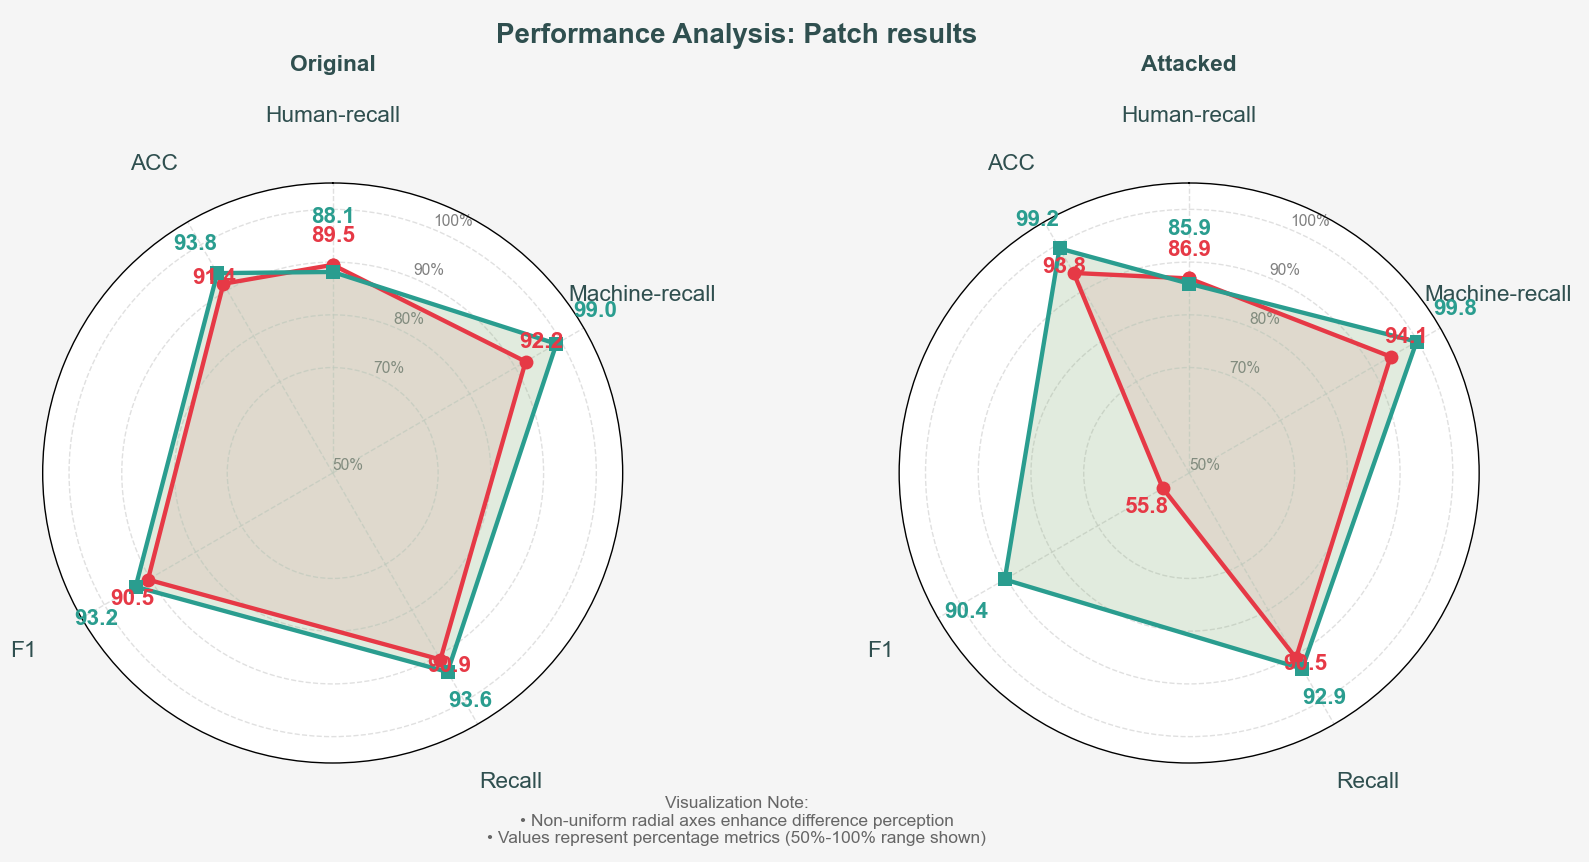
\includegraphics[width=\linewidth]{pics/patch-results.png}
    \caption{Illustration of "patch" result on supervised contrastive learning.}
\label{fig:patch_result}
\end{figure*}


\begin{table*}[ht]
	\centering
	\resizebox{0.8\textwidth}{!}{ 
	\renewcommand{\arraystretch}{1.1}
	\begin{tabular}{llccccc}
	\toprule
	\multirow{2}{*}{Type} & \multirow{2}{*}{Detectors} & \multicolumn{5}{c}{Metrics} \\
	\cmidrule(lr){3-7}
	& & Human-recall & Machine-recall & Recall & F1 & ACC \\
	\midrule
	
	\multirow{2}{*}{Original} 
	& Single & 88.11 & 87.54 & 87.82 & 88.78 & 88.77 \\
	& Patch & 96.94 & 84.56 & 90.75 & 97.30 & 95.33 \\
	& Joint & \cellcolor{yellow!50}88.35 & \cellcolor{yellow!50}98.08 & \cellcolor{yellow!50}93.22 & \cellcolor{yellow!50}92.22 & \cellcolor{yellow!50}92.92\\
	\cline{1-7}
	
	\multirow{2}{*}{Humanized}
	& Single & 86.55 & 90.61 & 88.58 & 70.21 & 90.52 \\
	& Patch & 98.88 & 99.01 & 98.94 & 98.32 & 98.96 \\ 
	& Joint &\cellcolor{yellow!50}88.55 & \cellcolor{yellow!50}99.91 & \cellcolor{yellow!50}94.23 & \cellcolor{yellow!50}92.37 & \cellcolor{yellow!50}99.35  \\
	
	\bottomrule
	\end{tabular}
	}
	\caption{Performance results of "patching" results of SimpleAI.}
	\label{tab:patch_results_SimpleAI}
	\end{table*}

	\begin{table*}[ht]
		\centering
		\resizebox{0.8\textwidth}{!}{ 
		\renewcommand{\arraystretch}{1.1}
		\begin{tabular}{llccccc}
		\toprule
		\multirow{2}{*}{Type} & \multirow{2}{*}{Detectors} & \multicolumn{5}{c}{Metrics} \\
		\cmidrule(lr){3-7}
		& & Human-recall & Machine-recall & Recall & F1 & ACC \\
		\midrule
		
		\multirow{2}{*}{Original} 
		& Single & 68.77 & 57.75 & 63.26 & 63.01 & 63.04 \\
		& Patch & 98.64 & 98.18 & 98.41 & 98.71 & 98.45 \\
		& Joint & \cellcolor{yellow!50}70.83 & \cellcolor{yellow!50}99.23 & \cellcolor{yellow!50}85.03 & \cellcolor{yellow!50}80.43 & \cellcolor{yellow!50}84.15\\
		\cline{1-7}
		
		\multirow{2}{*}{Humanized}
		& Single & 80.84 & 64.58 & 72.47 & 75.35 & 61.94 \\
		& Patch & 97.20 & 99.77 & 98.48 & 97.46 & 99.54 \\ 
		& Joint &\cellcolor{yellow!50}82.00 & \cellcolor{yellow!50}99.91 &\cellcolor{yellow!50} 90.96 & \cellcolor{yellow!50}89.17 & \cellcolor{yellow!50}99.11  \\
		
		\bottomrule
		\end{tabular}
		}
		\caption{Performance results of "patching" results of RADAR.}
		\label{tab:patch_results_RADAR}
		\end{table*}
		Similarly, we add our patch (subdivision layer) to the baseline detectors SimpleAI and RADAR, the results are shown in Tables \ref{tab:patch_results_SimpleAI} and \ref{tab:patch_results_RADAR}. In the table, single represents the result without using the patch, patch represents the further screening effect of our patch on the filtered human text, and joint represents the final effect of the detector after using the patch. It can be seen that after using our patch, all metrics of detectors have achieved breakthroughs (the yellow part in the table). Taking the F1 score as an example, for Task 1, the two detectors still have steady improvements, SimpleAI from 88.78\% to 92.22\%, an increase of 3.44\%; RADAR from 63.01\% to 80.43\%, an increase of 17.42\%. Furthermore, when facing humanized data sets, the performance improvement is particularly obvious, such as SimpleAI's F1 from 70.21\% to 92.37\%, a huge leap of 22.16\%. The above results show that our patch has well blocked the loophole that humanized machine text escapes detection after one screening. This patch is undoubtedly an extremely useful remedial tool for existing AI text detectors, and it also confirms the wide impact of our method.
\end{document}
